\documentclass{article}

\usepackage{hyperref}
\usepackage{graphicx}
\usepackage[labelformat=empty]{caption}

\setlength{\parindent}{0pt}

\title{Assembly Guide}
\author{D-Lab Team Mexico}

\begin{document}

\maketitle

\section{Software}
\subsection{Installing the Arduino IDE}
To install the Arduino IDE, visit the official Arduino website at the following link:

\href{https://www.arduino.cc/en/software}{https://www.arduino.cc/en/software}

\noindent
Download the version appropriate for your operating system and follow the installation instructions provided on the website.

\subsection{Installing the libraries}


Once you have opened the Arduino IDE, click on the Library Manager in the left bar. It has the following icon:

\vspace{1em}
\begin{center}
    
\includegraphics[width=0.2\textwidth]{../images/library_manager.png}
\end{center}

Now look for the following libraries:

\begin{itemize}
    \item Adafruit GFX Library, by Adafruit: say yes to installing all dependencies (which will be only Adafruit BusIO).
    \item MCUFRIEND\_kbv, by David Prentice.
    \item SD, by Arduino and SparkFun.
\end{itemize}

\noindent
Now, navigate to the location of your computer where the Arduino IDE keeps the Arduino Sketchbook folder. If you're unsure about where it is, there are some common paths:

\begin{itemize}
    \item Windows: C:\textbackslash Users\textbackslash [your username]\textbackslash Documents\textbackslash Arduino
    \item Mac: \(\sim \)/Documents/Arduino
    \item Linux: \(\sim \)/Arduino
\end{itemize}

Inside that folder, look for the folder "libraries". Click on "MCUFRIEND\_kbv" and then on "utils". Now, do the following:

\begin{itemize}
    \item Edit \texttt{mcufriend\_shield.h}: in the first line, remove the two slashes (\texttt{//}) before \texttt{\#define USE\_SPECIAL}.
    \begin{figure}[h]
        \centering
        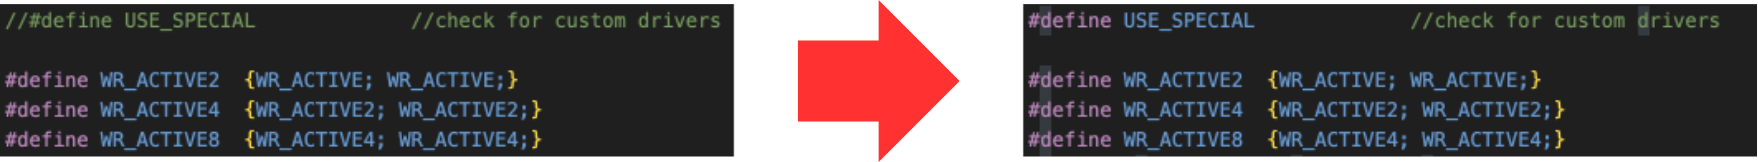
\includegraphics[width=1.3\textwidth]{../images/mcufriend_shield.png}
        \end{figure}
    \item Edit \texttt{mcufriend\_special.h}: in the 6th line, remove the two slashes (\texttt{//}) before \texttt{\#define USE\_MEGA\_16BIT\_SHIELD}.
\end{itemize}

\subsection{Downloading the code}
To download the code, go to the following link:

\href{https://github.com/CarolinaMoura/assistive-voices}{https://github.com/CarolinaMoura/assistive-voices}

Once in the page, click on the green button that reads "Code", and then on "Download ZIP":

\begin{figure}[h]
\centering

\includegraphics[width=0.3\textwidth]{../images/code.png}
\caption{The "code" button.}
\end{figure}

\begin{figure}[h]
\centering
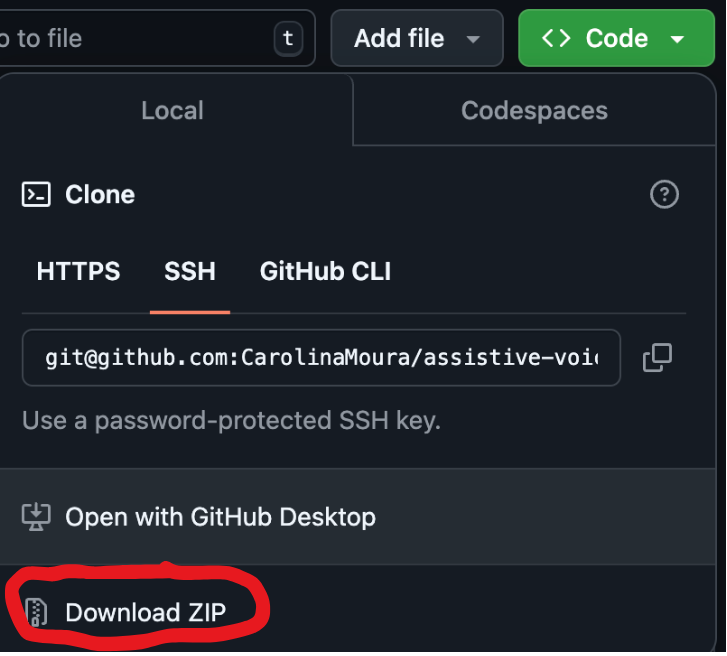
\includegraphics[width=0.5\textwidth]{../images/download_zip.png}
\caption{The "Download ZIP" option.}
\end{figure}

Now, unzip the downloaded folder. Inside the unzipped folder, you will find a folder named "main". This folder contains the code for the project.

\begin{itemize}
    \item Go inside the "main" folder.
    \item Double-click the file named "main.ino". This should open the Arduino IDE with the code.
    \item If the file does not open automatically, right-click on "main.ino" and select "Open with...". Choose the Arduino IDE from the list of available programs.
\end{itemize}

Now you have the code open in the Arduino IDE.

\section{Tools and Materials}
% List of tools and materials needed.

\section{Step-by-Step Instructions}
% Detailed assembly instructions.

\section{Troubleshooting}
% Common issues and solutions.

\section{Conclusion}
% Final remarks and tips.

\end{document}